%%%----------------------------------------------------------
\chapter{Distinctive Feature Tracking with SIFT (Option B)}
%%%----------------------------------------------------------

In this assignment the goal was to track a single feature over a sequence of successive frames and attach a graphic tag.

\section{Algorithm}
Similar to the last assignment \ref{chap:sift} the first step to track a feature is to use a SIFT detector. It returns a list of detected features which were inside of the selected region of interest in the first frame. The most dominant feature is selected and used as a reference feature in the next frame. In the upcoming frames the following steps are repeated:
\begin{enumerate}
	\item Use a SIFT detector to extract all features of the current frame.
	\item Find a feature matching the most dominant feature of the previous frame using a SIFT matcher.
	\item The selected feature is marked in the frame.
\end{enumerate}

\section{Process}
At first the region of interest had to be extracted from the image stack and map it to the image processor of the first frame. Then the SIFT features of the region of interest in the first frame were detected and the most dominant feature is stored. For each following frame the features are detected and then the \texttt{SiftMatcher} is used to match the most dominant feature of the last frame vs the features of the current frame. If a match is found it is memorized as the new most dominant feature and will be used for the next frame. If no match is found the old most dominant feature is used in the next frame. In each frame the current most dominant feature gets marked and the image is saved to the \texttt{resultImageStack} which is shown at the end.

\section{Results}
The algorithm produced only good results when there were only small changes between frames. As soon as it lost the feature once it had a really hard time finding it again. In the example in figure \ref{fig:11_1} the feature was tracked for the first couple frames but after the car went half offscreen after figure \ref{fig:11_3} it lost the feature and did not really find it again.

\begin{figure}
	\centering
	\begin{minipage}[t]{0.32\linewidth}
		\centering
		\frame{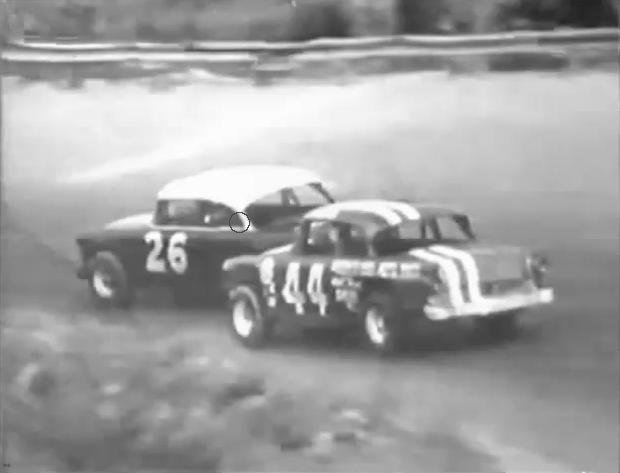
\includegraphics[width=.98\linewidth]{images/DrivingPassion_output1}}
		\caption{The tracked feature marked with a black circle.}
		\label{fig:11_1}
	\end{minipage}
	\hfill
	\begin{minipage}[t]{0.32\linewidth}
		\centering
		\frame{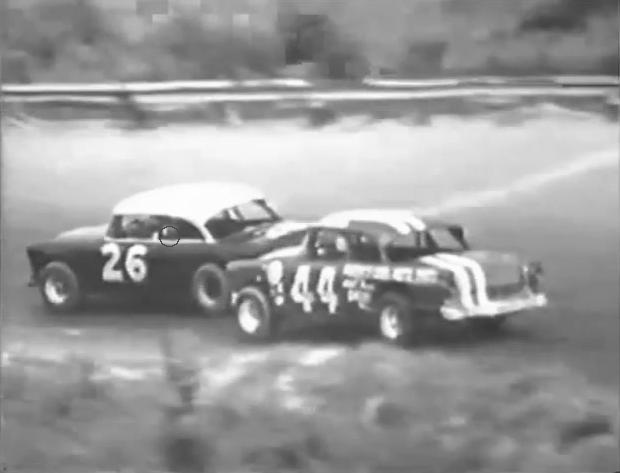
\includegraphics[width=.98\linewidth]{images/DrivingPassion_output2}}
		\caption{Feature tracking was stable so far.}
	\end{minipage}
	\hfill
	\begin{minipage}[t]{0.32\linewidth}
		\centering
		\frame{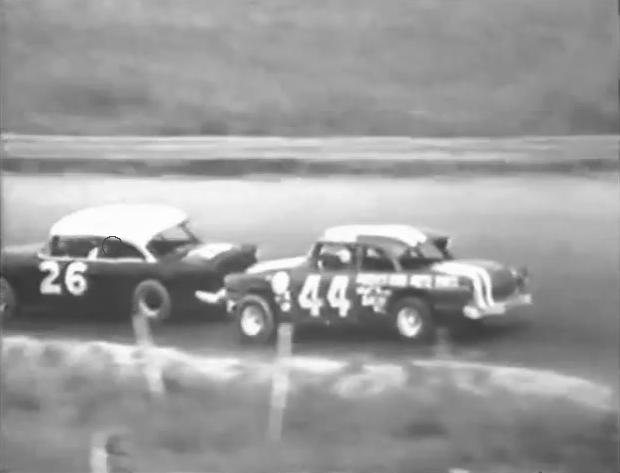
\includegraphics[width=.98\linewidth]{images/DrivingPassion_output3}}
		\caption{After the car went half offscreen the feature was lost and the algorithm had a hard time finding it again.}
		\label{fig:11_3}
	\end{minipage}
\end{figure}